\documentclass{article}
%\usepackage{fullpage}
%\usepackage[top=1in, bottom=1in, left=1cm,right=1cm]{geometry}
 \usepackage{geometry}
 \geometry{left=2.3 cm,right=2.3 cm,top=2 cm,bottom=2.1 cm}
\usepackage{fancyhdr}
\usepackage{color}
\usepackage[colorlinks,urlcolor={blue}]{hyperref}
\usepackage{amsmath}
%\usepackage[section]{placeins}
\usepackage{longtable}
\usepackage{lscape}
\usepackage{tikz}
\usetikzlibrary{trees}
\usepackage{amsmath}
\usepackage{float}
\usepackage{graphicx}
\usepackage{listings}
\usepackage{amsmath}
\begin{document}

\fancyfoot[L]{University of Michigan}
\fancyfoot[R]{Thomas Tian}
\pagestyle{fancyplain}


\title{\textbf{Behavioral Cloning Report}}
\author{Thomas Tian}

\maketitle


\section{Project Introduction}

In this project, I used what I've learned about deep neural networks and convolutional neural networks to clone driving behavior. I trained, validated and tested a model using Keras. The model outputs a steering angle to an autonomous vehicle.

I used a simulator provided by Udacity where I can steer a car around a track for data collection. I used image data and steering angles to train a neural network and then used this model to drive the car autonomously around the track.

\section{Data Collection and Pre-Processing}

The training data set was obtained by manually operating an vehicle in the simulator provided by the Udaciy. Three images were captured when the vehicle runs on the track at each time index. Figure~\ref{fig: center}, Figure \ref{fig: left} and Figure \ref{fig: right} show the three view images captured by the cameras. Note that all three images have the same associated steer angle, how ever, I added an angle offset, $\delta_S = 0.2 ^o$ and $\delta_S = -0.2 ^o$ to the left and right camera view, respectively, to generate more data. Moreover, the all the images are flipped and the corresponding steering angle is multiplied by $-1$ to generate more data. Therefore, the number of the total training images can be calculated by
\begin{equation}
N = 2*n,
\end{equation}   
where n is the number of the images captured. To generalize the training model and make the vehicle have the ability to steer back when it deviates from the center of the track, the data I obtained by manually driving the vehicle is augmented with training set provided by Udacity to make the training more effective. 

The image I got from the camera has more than enough information I need to predict the steering angle, such as the front of the vehicle, sky. Therefore, all the images are cropped (70 pixels from the top and 20 pixels from the bottom) to eliminate the extra information. Moreover, all the images's brightness level (HSV) in the data set are randomly adjusted to generate more data. 


\begin{figure}[!ht]
\centering
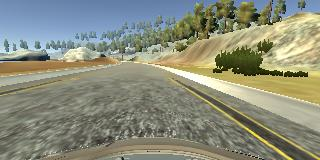
\includegraphics[width=0.4\textwidth]{center.JPG}
\caption{Center camera view.}
\label{fig: center}
\end{figure}
\begin{figure}[!ht]
\centering
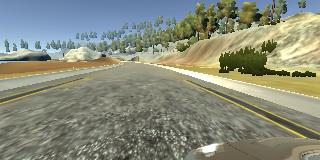
\includegraphics[width=0.4\textwidth]{left.JPG}
\caption{Left camera view.}
\label{fig: left}
\end{figure}
\begin{figure}[H]
\centering
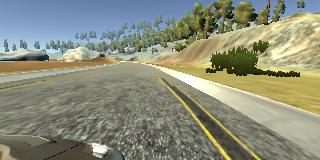
\includegraphics[width=0.4\textwidth]{right.JPG}
\caption{Right camera view.}
\label{fig: right}
\end{figure}

\section{Model Architecture and Training Strategy}
\subsection{Model Architecture}

A deep neural network was employed to train the model. Figure~\ref{fig: cnn} shows the structure of the used CNN. The model I used is a modified version from the NVIDIA CNN model. The NVIDIA has proven to be a excellent model for image classification and prediction, thus I used this model as a start point. In practice, I added two additional fully connected followed by dropout to prevent over fitting, which improved the accuracy a little. 

\begin{figure}[H]
\centering
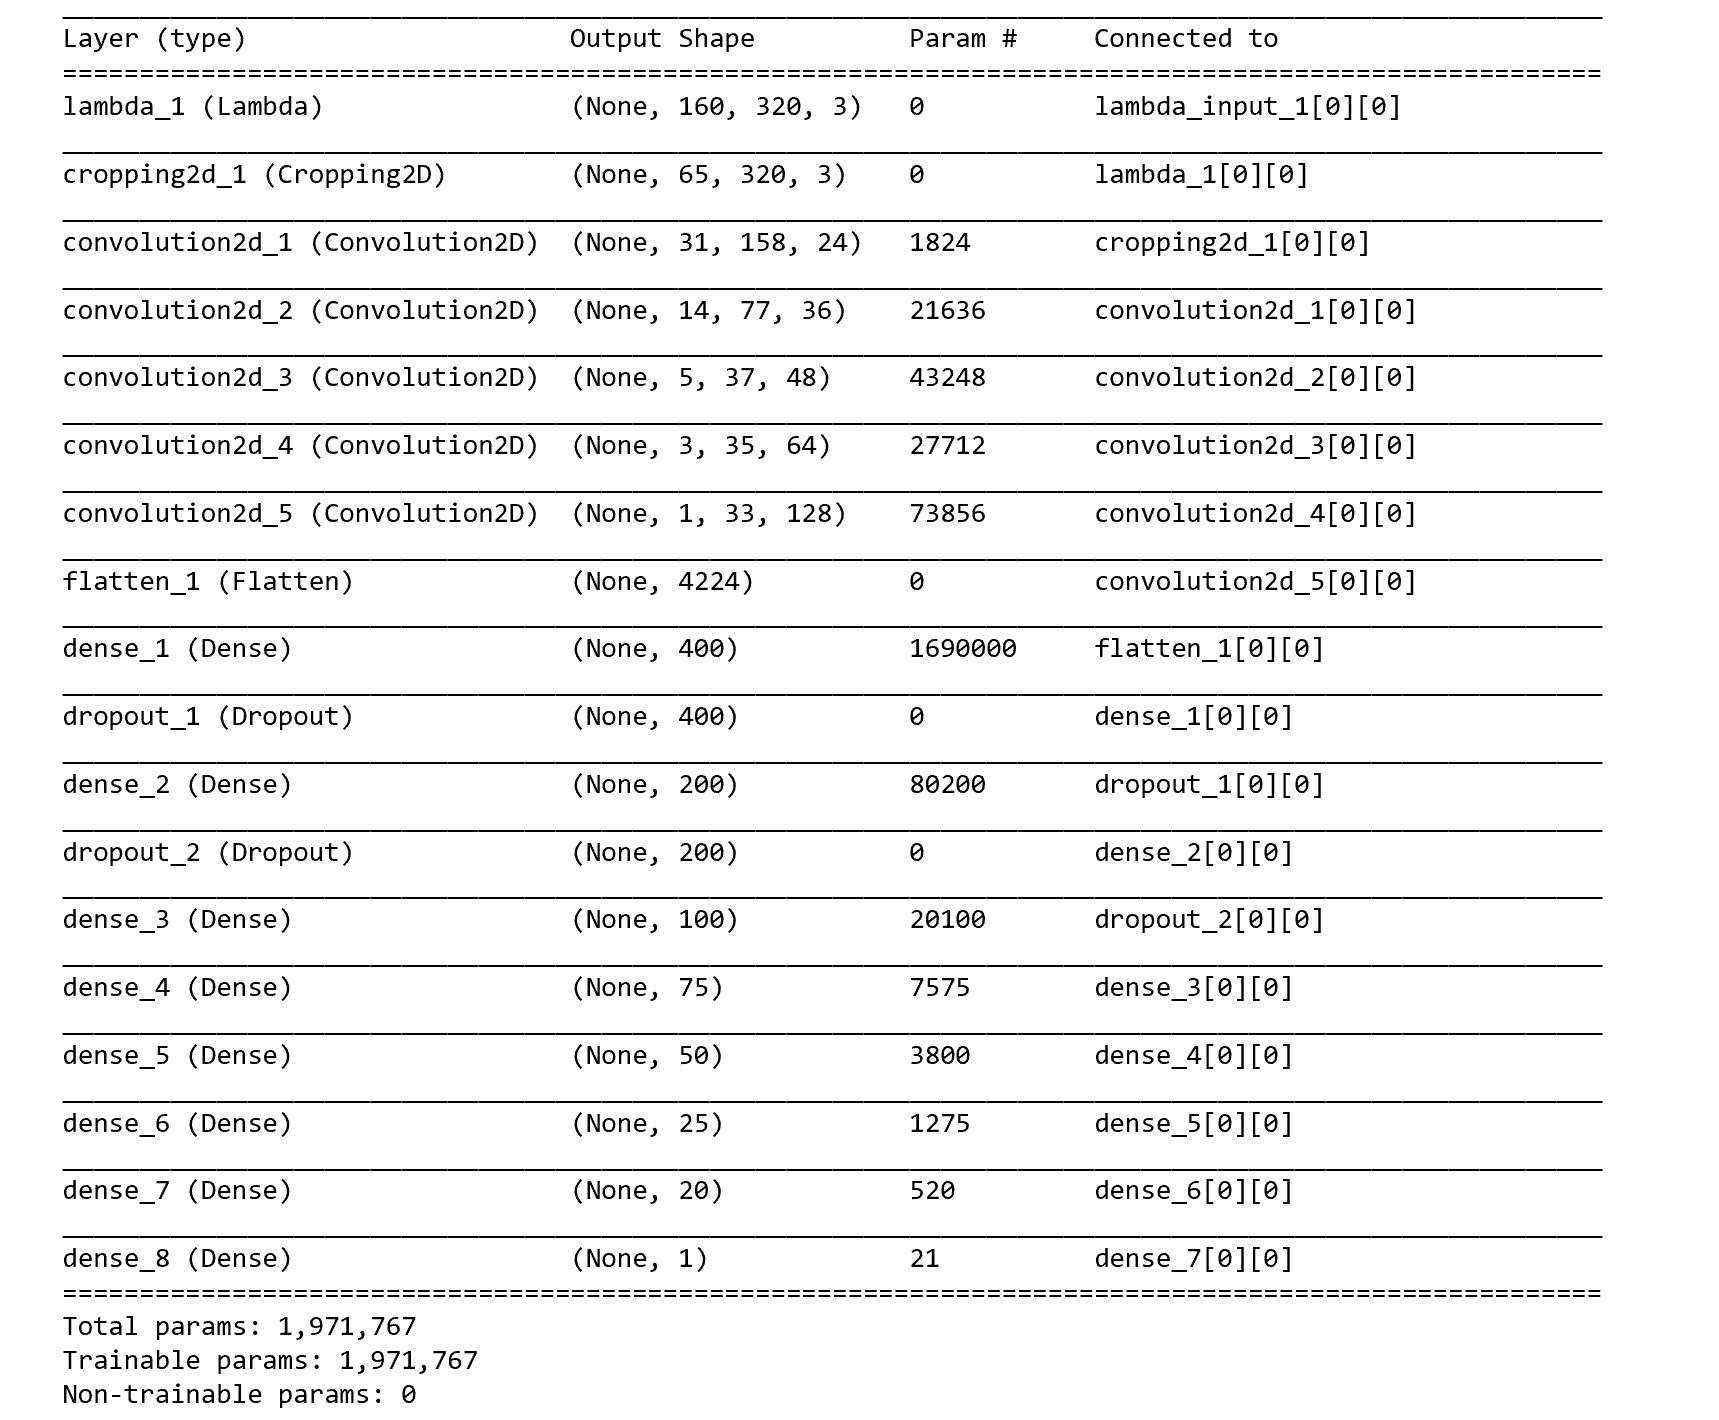
\includegraphics[width=0.6\textwidth]{cnn_model.png}
\caption{CNN model.}
\label{fig: cnn}
\end{figure}

\subsection{Training Strategy}
The collected images were shuffled and split into two sets, training set and validation set. The training set contains $80\%$ of the collected data and the validation set contains $20\%$ of the collected data. Since the amount of the training data is significantly larger compared with the training data in the traffic sign classifier project, thus a data generator was implemented to generate data as the training process needed. The training uses an Adam optimizer so that the learning rate is determined by the optimizer. Four training Epochs were used until the training was completed. 


\section{Training Result}
I trained the model with different camera views and noticed that the accuracy using only center camera images for training, $60\%$, is much larger than the accuracy using images from three cameras, $30\%$. However, when testing the trained model in the simulator, the model trained with all three cameras' images showed better performance as the vehicle has the ability to steer back when it deviates from the center. The demovideo.mp4 shows the vehicle running on the track using trained model.

\begin{figure}[H]
\centering
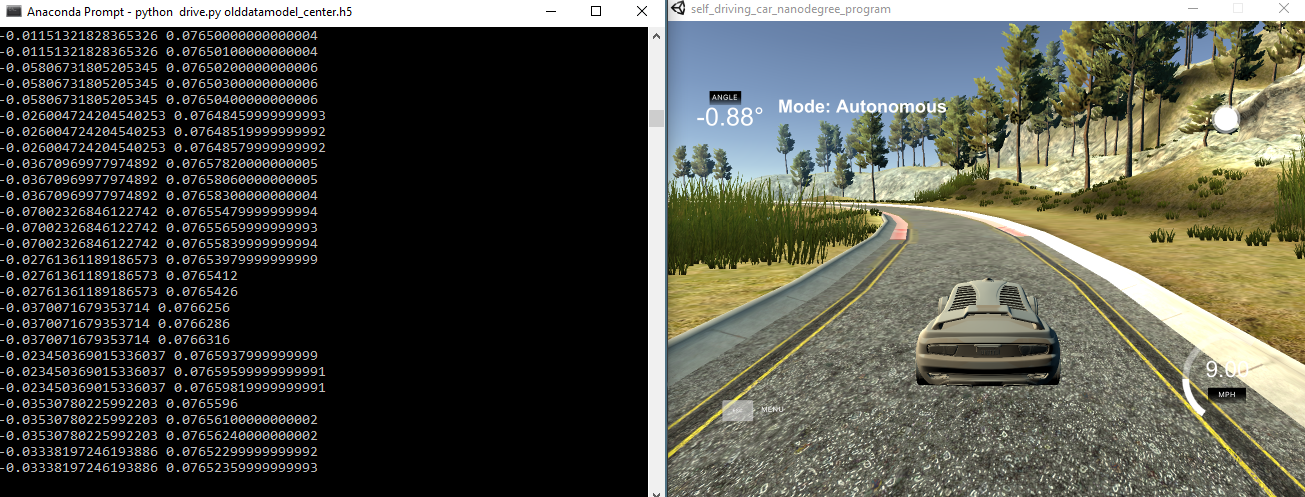
\includegraphics[width=0.9\textwidth]{demo.PNG}
\caption{Vehicle running in autonomous mode.}
\label{fig: cnn}
\end{figure} 




\end{document}
